\documentclass[a4paper,english,abstract=on]{scrartcl}

\usepackage{mathtools} % loads amsmath and fixes its bugs in Unicode & XeLaTeX/LuaLaTeX 
\usepackage[english]{babel}
\usepackage[]{unicode-math} % provides Unicode Math support for XeLaTeX/LuaLaTeX 
\usepackage{xcolor}
\usepackage{graphicx}
\usepackage[pdfborder={0 0 0}]{hyperref}
\usepackage[autostyle=true]{csquotes}
\usepackage[backend=biber, style=numeric-comp]{biblatex}
\addbibresource{literatur.bib}
\usepackage{listings}
\lstset{language=SQL}

\title{Exercise 2 Report}
\subtitle{Gruppe 16}
\author{Anastasiia Rubanovych\and Sebastian Funck}
\date{\today}

\begin{document}

\maketitle

\section{SQL commands to create the schema}
\begin{lstlisting}{Name}
CREATE SCHEMA estatesmgmt AUTHORIZATION root;

CREATE TABLE estatesmgmt.apartments (
fk_estate_id int4 NOT NULL,
balcony bool NOT NULL DEFAULT false,
kitchen bool NOT NULL DEFAULT false,
room int4 NOT NULL,
floor int4 NOT NULL,
rent float4 NOT NULL,
CONSTRAINT apartment_pk 
    PRIMARY KEY (fk_estate_id),
CONSTRAINT fk_estates 
    FOREIGN KEY (fk_estate_id) 
    REFERENCES estatesmgmt.estates(id) 
    ON UPDATE CASCADE 
    ON DELETE CASCADE
);

CREATE TABLE estatesmgmt.contracts (
id serial NOT NULL,
"date" date NOT NULL,
place varchar NOT NULL,
fk_person_id int4 NOT NULL,
CONSTRAINT contract_pk 
    PRIMARY KEY (id),
CONSTRAINT contracts_fk 
    FOREIGN KEY (fk_person_id) REFERENCES estatesmgmt.persons(id)
);

CREATE TABLE estatesmgmt.estate_agents (
name varchar NOT NULL,
address varchar NOT NULL,
login varchar NOT NULL,
"password" varchar NOT NULL,
id serial NOT NULL,
CONSTRAINT estate_agent_pk 
    PRIMARY KEY (id),
CONSTRAINT estate_agent_un 
    UNIQUE (login)
);

CREATE TABLE estatesmgmt.estates (
id serial NOT NULL,
city varchar NOT NULL,
postal_code int4 NOT NULL,
street varchar NOT NULL,
street_number int4 NOT NULL,
square_area int4 NOT NULL,
fk_estate_agent_id int4 NOT NULL,
CONSTRAINT estate_pk 
    PRIMARY KEY (id),
CONSTRAINT fk_estate_agents 
    FOREIGN KEY (fk_estate_agent_id) 
    REFERENCES estatesmgmt.estate_agents(id)
);

CREATE TABLE estatesmgmt.houses (
number_of_floors int4 NOT NULL,
price float4 NOT NULL,
garden bool NOT NULL DEFAULT false,
fk_estate_id int4 NOT NULL,
CONSTRAINT house_pk 
    PRIMARY KEY (fk_estate_id),
CONSTRAINT fk_estates 
    FOREIGN KEY (fk_estate_id) 
    REFERENCES estatesmgmt.estates(id) 
    ON UPDATE CASCADE 
    ON DELETE CASCADE
);

CREATE TABLE estatesmgmt.persons (
id serial NOT NULL,
first_name varchar NOT NULL,
last_name varchar NOT NULL,
address varchar NOT NULL,
CONSTRAINT person_pk PRIMARY KEY (id)
);

CREATE TABLE estatesmgmt.purchase_contracts (
number_of_installment int4 NOT NULL DEFAULT 1,
interest_rate float4 NULL,
fk_contract_id int4 NOT NULL,
fk_house_id int4 NOT NULL,
CONSTRAINT purchase_contract_pk 
    PRIMARY KEY (fk_contract_id),
CONSTRAINT fk_houses 
    FOREIGN KEY (fk_house_id) 
    REFERENCES estatesmgmt.houses(fk_estate_id),
CONSTRAINT purchase_contract_fk 
    FOREIGN KEY (fk_contract_id) 
    REFERENCES estatesmgmt.contracts(id)
    ON DELETE CASCADE
);

CREATE TABLE estatesmgmt.rents (
apartment_id int4 NOT NULL,
person_id int4 NOT NULL,
tenancy_contract_id int4 NOT NULL,
CONSTRAINT rents_apartment_1 UNIQUE (apartment_id),
CONSTRAINT rents_contract_1 UNIQUE (tenancy_contract_id),
CONSTRAINT rents_pk 
    PRIMARY KEY (apartment_id, person_id, tenancy_contract_id),
CONSTRAINT rents_fk_apartment 
    FOREIGN KEY (apartment_id) 
    REFERENCES estatesmgmt.apartments(fk_estate_id),
CONSTRAINT rents_fk_contract
    FOREIGN KEY (tenancy_contract_id) 
    REFERENCES estatesmgmt.tenancy_contracts(fk_contract_id),
CONSTRAINT rents_fk_person 
    FOREIGN KEY (person_id) 
    REFERENCES estatesmgmt.persons(id)
);

CREATE TABLE estatesmgmt.tenancy_contracts (
start_date date NOT NULL DEFAULT CURRENT_DATE,
duration interval NOT NULL,
additional_cost float4 NOT NULL DEFAULT 0,
fk_contract_id int4 NOT NULL,
fk_apartment_id int4 NOT NULL,
CONSTRAINT tenancy_contract_pk 
    PRIMARY KEY (fk_contract_id),
CONSTRAINT fk_apartment_id 
    FOREIGN KEY (fk_apartment_id) 
    REFERENCES estatesmgmt.apartments(fk_estate_id),
CONSTRAINT tenancy_contract_fk 
    FOREIGN KEY (fk_contract_id) 
    REFERENCES estatesmgmt.contracts(id) 
    ON DELETE CASCADE
);
\end{lstlisting}

\section{Create an apartment, an estate agent and a tenancy contract with your java application. Validate that they are in the database.}
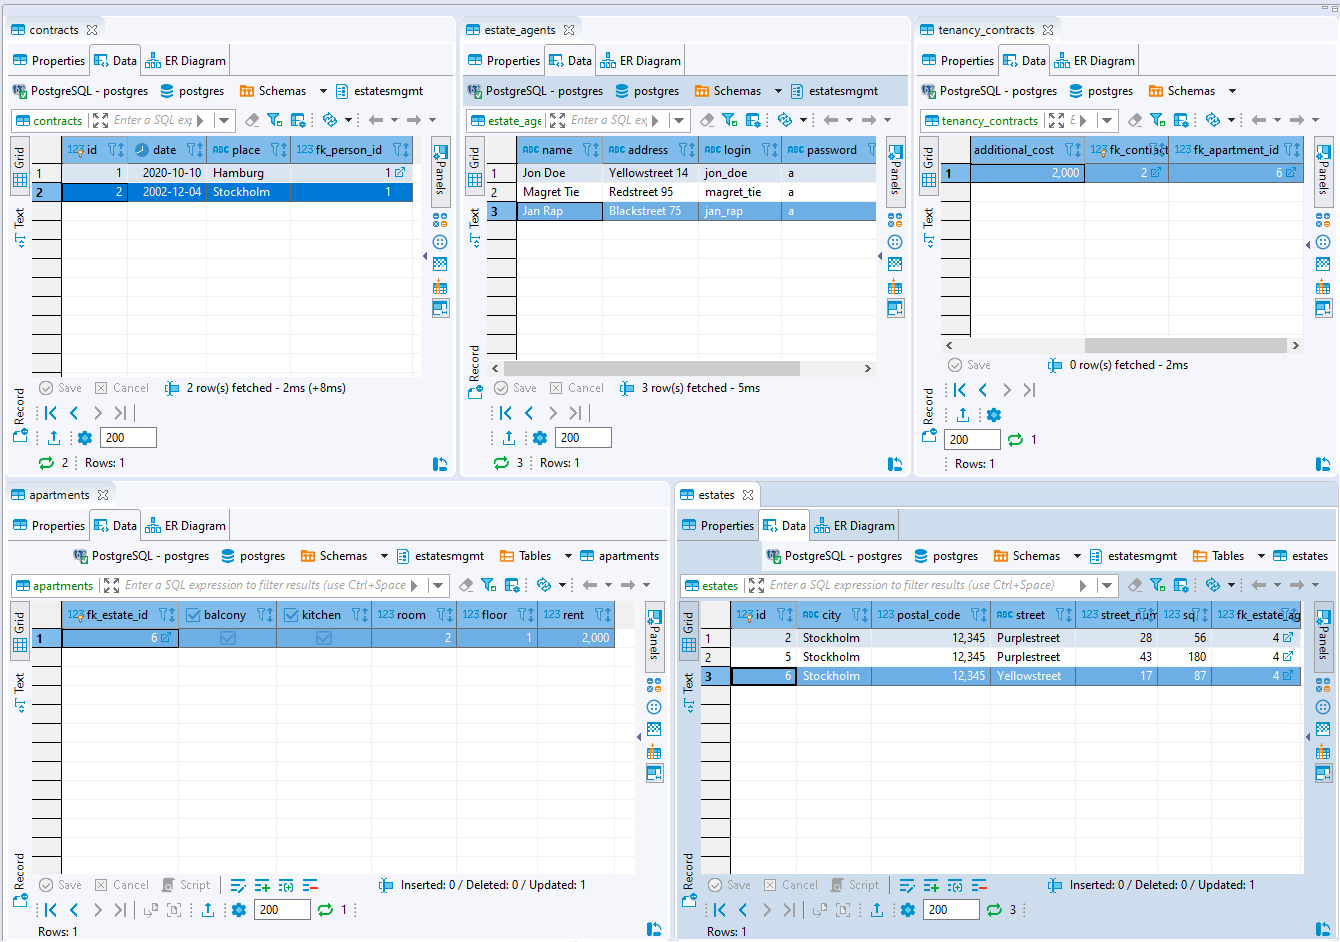
\includegraphics[scale=0.4]{tenacy_contract.png}

\section{Create a contract with a non-existing estate. Does it work? Why/Why not?}
It doesn't work, because it violates the \texttt{NOT NULL} property of \texttt{fk\_estate\_id} and the foreign key of \texttt{contracts} that requires an existing estate.

\section{Which inheritance model did you choose and why?}
We chose the vertical inheritance model because modifying a base class will be easier, as it won't required to modify any of the subclasses. Subclasses only contain the fields they add to the base class.

\section{Create an apartment, and let your application crash between inserting the estate information and inserting the apartment information. What is the effect on your database state?}
Only the estate entry is created, but it has neither a house nor an apartment entry.

\printbibliography
\end{document}
